\chapter{Systematic Uncertainties}
\label{chapter:systematics}
\minitoc
The data driven background estimation and using the ratio of the number of signal region events to control region events eliminates the systematic uncertainties related to potential mismodeling of the tails of kinematic distributions such as $\LT$, $\HT$, $\DF$. However, there are still several sources that can affect the background prediction and expected signal events counts. These sources and the methods to calculate the uncertainties are discussed in the following.
\section{Systematic uncertainties on background estimation}
These sources and the methods to calculate the uncertainties are discussed in the following.
Because the $\kappa$ factors of the analysis are taken from simulation, these factors are reflecting the influence of mismodeling of the $\Rcs$ and hence the fractions of background processes on the analysis. Therefore, the systematic uncertainties on the background estimation are calculated through $\kappa_{\ttbar}$ and $\kappa_{w}$.  The amount of uncertainty is then determined as:
\begin{equation}
\label{eqn:syst_unc_kappa}
\delta = \frac{\kappa _x'}{\kappa _x}-1\, ,
\end{equation}
where $\kappa'$ reflects the recalculated $\kappa$ with varied weights and x stands for $\ttbar$ or $w$.\\
{\boldmath $\njet$} \textbf{extrapolation for}  {\boldmath $\ttbar+$} \textbf{jets:}\\
One of the major systematic uncertainties on the background estimate results from the extrapolation of $\Rcs$ from the measurement region, low $\njet$, to the application region, high $\njet$. This uncertainty can be calculated with a fit which is performed over the $\njet$ range as in Fig. \ref{RCS_dataMCw} (left).  The relative difference between the $\Rcs$ value obtained in the side band in simulated samples and the value derived from the fit is taken as a systematic uncertainty on $\wJets$ events.\\
The same procedure would also be applied for $\ttJets$ events as well. However, in this method limit statistics of some bins affects significantly the systematic uncertainty calculations. Therefore, another method is developed based on the impact of different fractions of dileptonic and single leptonic $\ttbar$ events. To account for this effect, as discussed in Sec. \ref{sec:RcsTT}, an event by event weight for correction factor $\kappa_{\ttbar}$, which is showned in Eq. \ref{weight_DL}, is derived.
In addition to this, two weights are obtained to calculate the systematic uncertainties originated from the procedure:
\begin{eqnarray}
W(DL_{\rm Const}) = 1\pm23\%,\\
W(DL_{\rm Slope}) = 1\pm(\njet-5.9) \cdot 5\%.
\end{eqnarray}
The variations are extracted as the quadratic sum of the deviation from 1 for the constant (offset) parameter and its uncertainty or as the quadratic sum of the deviation from 0 for the slope parameter and its uncertainty.
The uncertinities derived from the slope and constant variation as a fucntion of the $\kappa_{\ttbar}$ is shown in Fig. \ref{fig:systDL}. In this Figure, color filled areas represent the dilepton uncertinities while the black line shows the unceartinity calculated with fit along the $\njet$, which is not used in the analysis. The offset variation almost has no effect on $\kappa_{\ttbar}$ while the slope variation has an effect up to 20\%. The figure manifests that the two different approach result in the similar values of uncertainties while the uncertainty calculated with $\njet$ fit fluctuates to higher values the statistical effects. 
\begin{figure*}[!hbt]
    \begin{center}
 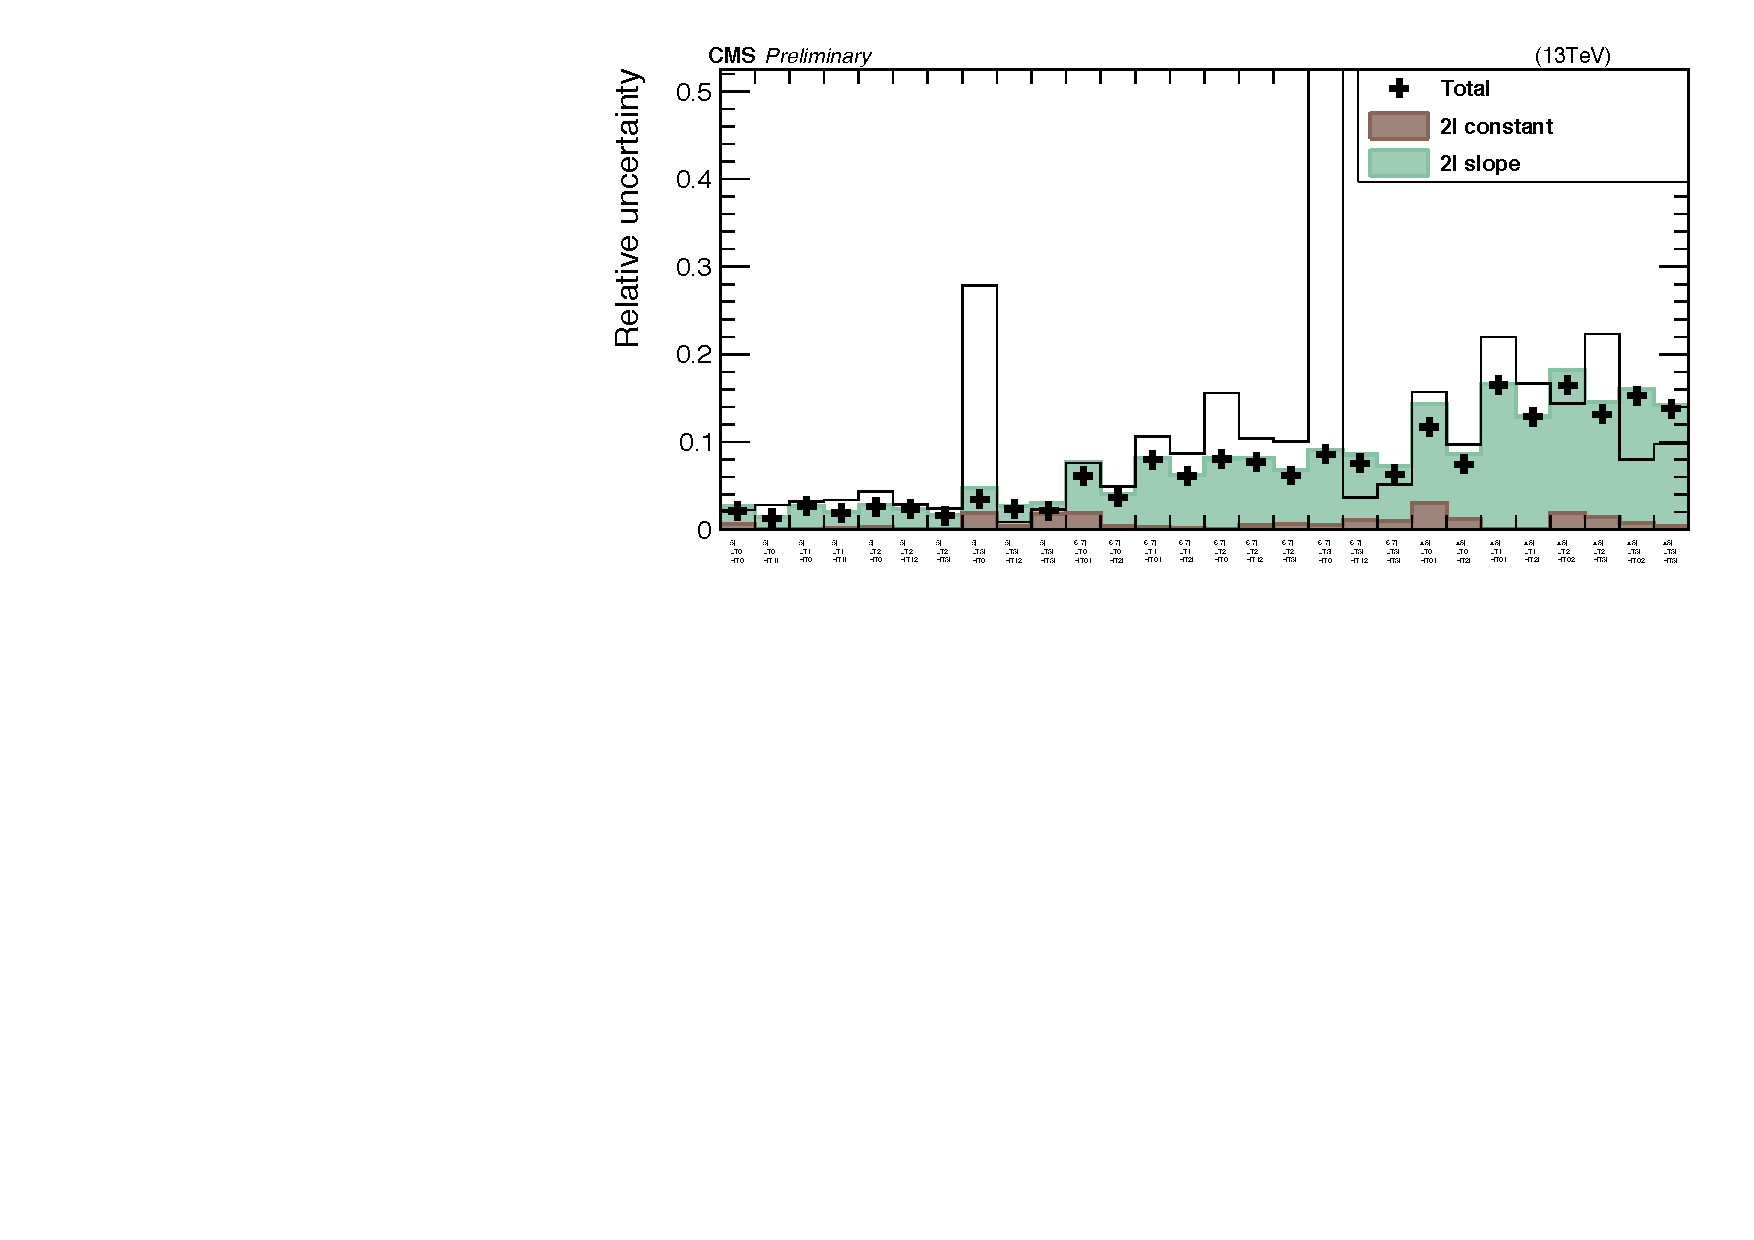
\includegraphics[width=0.8 \textwidth]{Plots/analysis/RCS/diLepCR/DL_comp}
  \caption{ \label{fig:systDL} Relative uncertinity on $\kappa_{\ttbar}$ due to the different composition of dileptonic events in sideband and main band regions. Color filled areas represent the dilepton uncertinities while the black line shows the unceartinity calculated with fit along the $\njet$.}
  \end{center}
\end{figure*}
\\
\textbf{Cross sections:}\\
To account for possible biases in the estimation of the background composition in terms of $\wJets$ vs. $\ttJets$ events, uncertainties on their cross sections are taken in to account. Although in the inclusive regions the $W$ boson cross section \cite{Wcross} and $\ttbar$ cross section \cite{ttcross} uncertainties are at the order of ten percent level, in the analysis regions it can be larger. The $\wJets$ and $\ttJets$ cross sections are conservatively varied by 30\%, which lead to a change 0.3-10\% (0.7-13\%) in the $\kappa_w$ ($\kappa_{\ttbar}$) values. \\
For other small EWK background processes, which are taken directly from simulation, again a conservative 50\% variation is applied. Because, the fraction of these events are small, the effect of this variation on the $\kappa$ values is calculated to be changing between 0.1-3.8\%.
\\
\textbf{W polarization:}\\
The main search variable $\DF$ reflects the angular information between the $W$ boson and its decay products. Therefore, the $W$ boson polarization affects the $\DF$ distribution. The effect of the polarization on background estimation of $\wJets$ and $\ttJets$ is calculated by reweighing these events by:
\begin{equation}
\label{eqn:W_pol}
w = (1 \pm a\cdot(1-cos(\theta^*)))\cdot C
\end{equation}
where a is 5\% for  $\ttJets$ and 10\% for $\wJets$ events, C is a factor to keep the normalization after baseline constant and $\theta*$ is the angle between the charged lepton and the W boson in the W rest frame. This procedure results in an uncertainty below 3\% in all the signal regions. \\
\textbf{number of ISR jets reweighting:}\\
In Sec. \ref{sec:SF}, the reweightenning of events according to number of ISR jets is already explained.
$\kappa$ values are recalculated by varying the ISR weights with the systematic uncertainties listed in Tab. \ref{tab:nISRweights}. The amount of variation is then calculated using the Eqn. \ref{eqn:syst_unc_kappa} and found to be varying between 0.2-11\%.\\
\textbf{QCD multijet events prediction:}\\
QCD multijet events prediction is entering in this search through the b-tag multiplicity fit (see Sec.\ref{sec:bkgcomp}) to measure the background compositions in control regions and also through  calculation of the $\Rcs$ values. Therefore the uncertainty originated from QCD prediction has to be considered. A profound explanation of the QCD prediction and its uncertainty can be found in \cite{David}.  The effect of this uncertainty is propagated to the $Rcs$ prediction. The resultant uncertainty is found to be around 3\%.\\
\textbf{$\Rcs$ difference muon/(electron or muon):}\\
As discussed in Sec. \ref{sec:RcsW}, $\Rcs$ of $\wJets$ events is calculated only in the muon channel. To account for the inconsistency between the $\Rcs$ with only muon channel and the true $\Rcs$, the discrepancy between these values are taken from the simulation. This discrepancy is assigned as systematic uncertainty. In order to avoid large uncertainties driven by the limited statistics, the systematic uncertainty is restricted to be smaller than the statistical error of the true $\Rcs$ value. 
\section{Systematic uncertainties on signal modelling}
The uncertainties considered in this section are applied only to the simulated signal events.  The amount of discrepancy is calculated as:
\begin{equation}
\label{eqn:syst_unc_signal}
\delta = \frac{N'_{\rm events}}{N_{\rm events}}-1\, ,
\end{equation}
where $N'_{\rm events}$ represents the recalculated number of simulated signal events with varied weights and $N_{\rm events}$ is the true number of events. The systematic uncertainties are calculated for each search bin separately as in the background case, this time uncertainties are also calculated for each 657 gluino/neutrino mass points. \\
\textbf{Initial state radiation:}\\
In Run 1 it was observed that the hadronic recoil from ISR for boosted heavy particle pairs such as the $\ttbar$ system is not well described by the $\MADGRAPH$ event generator \cite{ISR}. As a very similar system, it is expected that the gluino pair lead discrepancies.
An uncertainty based on the $\pt$ of the gluino-gluino system is applied:
\begin{itemize}
\item $\pt$ (gluino-gluino) less than 400 GeV: no uncertainty
\item $\pt$ (gluino-gluino) between 400 GeV and 600 GeV: 15\% uncertainty
\item $\pt$ (gluino-gluino) above 600 GeV: 30\% uncertainty.
\end{itemize}
The uncertainty on the number of expected signal events is calculated by varying each event with propagating the variations listed above through Eqn. \ref{eqn:syst_unc_signal}.\\
\textbf{Factorization/renormalization scale:}\\
To account for the impact of renormalization and factorization scales on the signal acceptance, the scales are varied by a factor of 0.5 and 2, respectively. As discussed in Sec. \ref{sec:simulation}, there are several weights to be applied for these scale factors. Therefore, to calculate the uncertainty an envelope of all variations is computed. Furthermore, to keep the cross section unchanged, a normalization factor is applied. The resultant uncertainty on the expected event yields is similar for all the mass points and it is changing between 1-3\%.
\textbf{Reconstruction of MET:} \\
On the recommendation of corridor studies group, the analysis is performed separately for reconstructed and generated MET, that is to recalculate all the kinematic variables, which include MET.  The average of the two acceptances is taken as the central value of the expected signal yields for each main band region. Furthermore, one-half of the difference between the two acceptances is taken as an uncertainty.\\
\textbf{Trigger:}\\
As introduced in Sec. \ref{sec:triggers}, the uncertainty on the trigger selection efficiency is measured to be around 2\%, and also considered as the uncertainty on signal simulation. \\
\textbf{Luminosity:}\\
As shown in Sec. \ref{sec:luminosity},  the pixel cluster counting method \cite{lumi1} is used to calculate luminosity. The uncertainty on this measurement is predicted to be 2.5\% \cite{lumi2}.\\
\section{Common systematic uncertainties for signal and background modelling}
Systematic uncertainties affecting both background and the signal processes are related to the mismeasurement misidentification of particular objects in the events. These uncertainties have impact on the kinematic variables of the analysis: $\DF$, $\LT$, $HT$, $\njet$, $\nbjet$. Therefore, for the signal events they are affecting the acceptance and the selection efficiency and for the background events they may vary the $\Rcs$ values.\\
\textbf{Jet Energy Scale:}\\
Calculating uncertainty on the jet energy scales is another dedicated study performed by JET-MET physics object group at CMS. Within the analysis, these variations which are affecting the jet energy spectrum as well as $\MET$, are applied to the jets in individual events and therefore related kinematic variables are reconstructed.
For the background estimate, $\kappa$ values are recalculated with up and down scaled jets. The uncertainty, which is obtained using Eqn. \ref{eqn:syst_unc_kappa}, is found to be changing between 0.7-26\%. For the signal, yields are recalculated and variation is measured using Eqn. $\ref{eqn:syst_unc_signal}$. In this case, depending on the mass point and signal region, uncertainty can take values up to 40\%.\\
\textbf{Tagging of b-jets:}\\
B-tagging uncertainties, which are related to difference in b-tagging efficiency between simulated and observed events, have an influence on this analysis through acceptance and b-tag multiplicity fit. Uncertainties are calculated to be less than 3\% for the background, and between 1-6\% for the signal.\\
\textbf{Lepton identification and reconstruction:}\\
Lepton identification and reconstruction efficiencies are different for simulated and observed events. For the backgrounds, a flat 5\% uncertainty is assigned to account for this difference. For signal, also variations originated from the difference between fast simulation \cite{FastSim} and full simulation are taken into account. The resultant uncertainty on the expected signal yields is found to be 2\%. \\
\textbf{Pileup:}\\
To cover the difference between the simulated pileup and data, the inelastic cross section is varied by 5\% up and down and the varied versions of Fig. \ref{fig:pileUpmine} is obtained. For the background the weights for up and down variations are propagated to the $\kappa$ calculation. For the signal, due to the fact that the signal yields in main band signal region do not significantly depend on pileup, simulation samples are not reproduced for the high pileup environment. In Fig. \ref{fig:pileUpdependence} y-axis is calculated as follows:
\begin{equation}
{\rm PU_{dependence}}= \frac{{\rm Efficiency_{high}} }{{\rm Efficiency_{low}} },
\end{equation}
where $\rm Efficiency_{high}$ and $\rm Efficiency_{low}$ is defined as in the Eqn. \ref{eff_PU}.
\begin{eqnarray}
\label{eff_PU}
{\rm Efficiency_{high}} = \frac{N(n_{\rm verticies}\geq20, MB)}{N(n_{\rm verticies}\geq20, baseline)},\\
{\rm Efficiency_{low}} = \frac{N(n_{\rm verticies}<20, MB)}{N(n_{\rm verticies}<20, baseline)}.
\end{eqnarray}
\begin{figure*}[!hbt]
    \begin{center}
 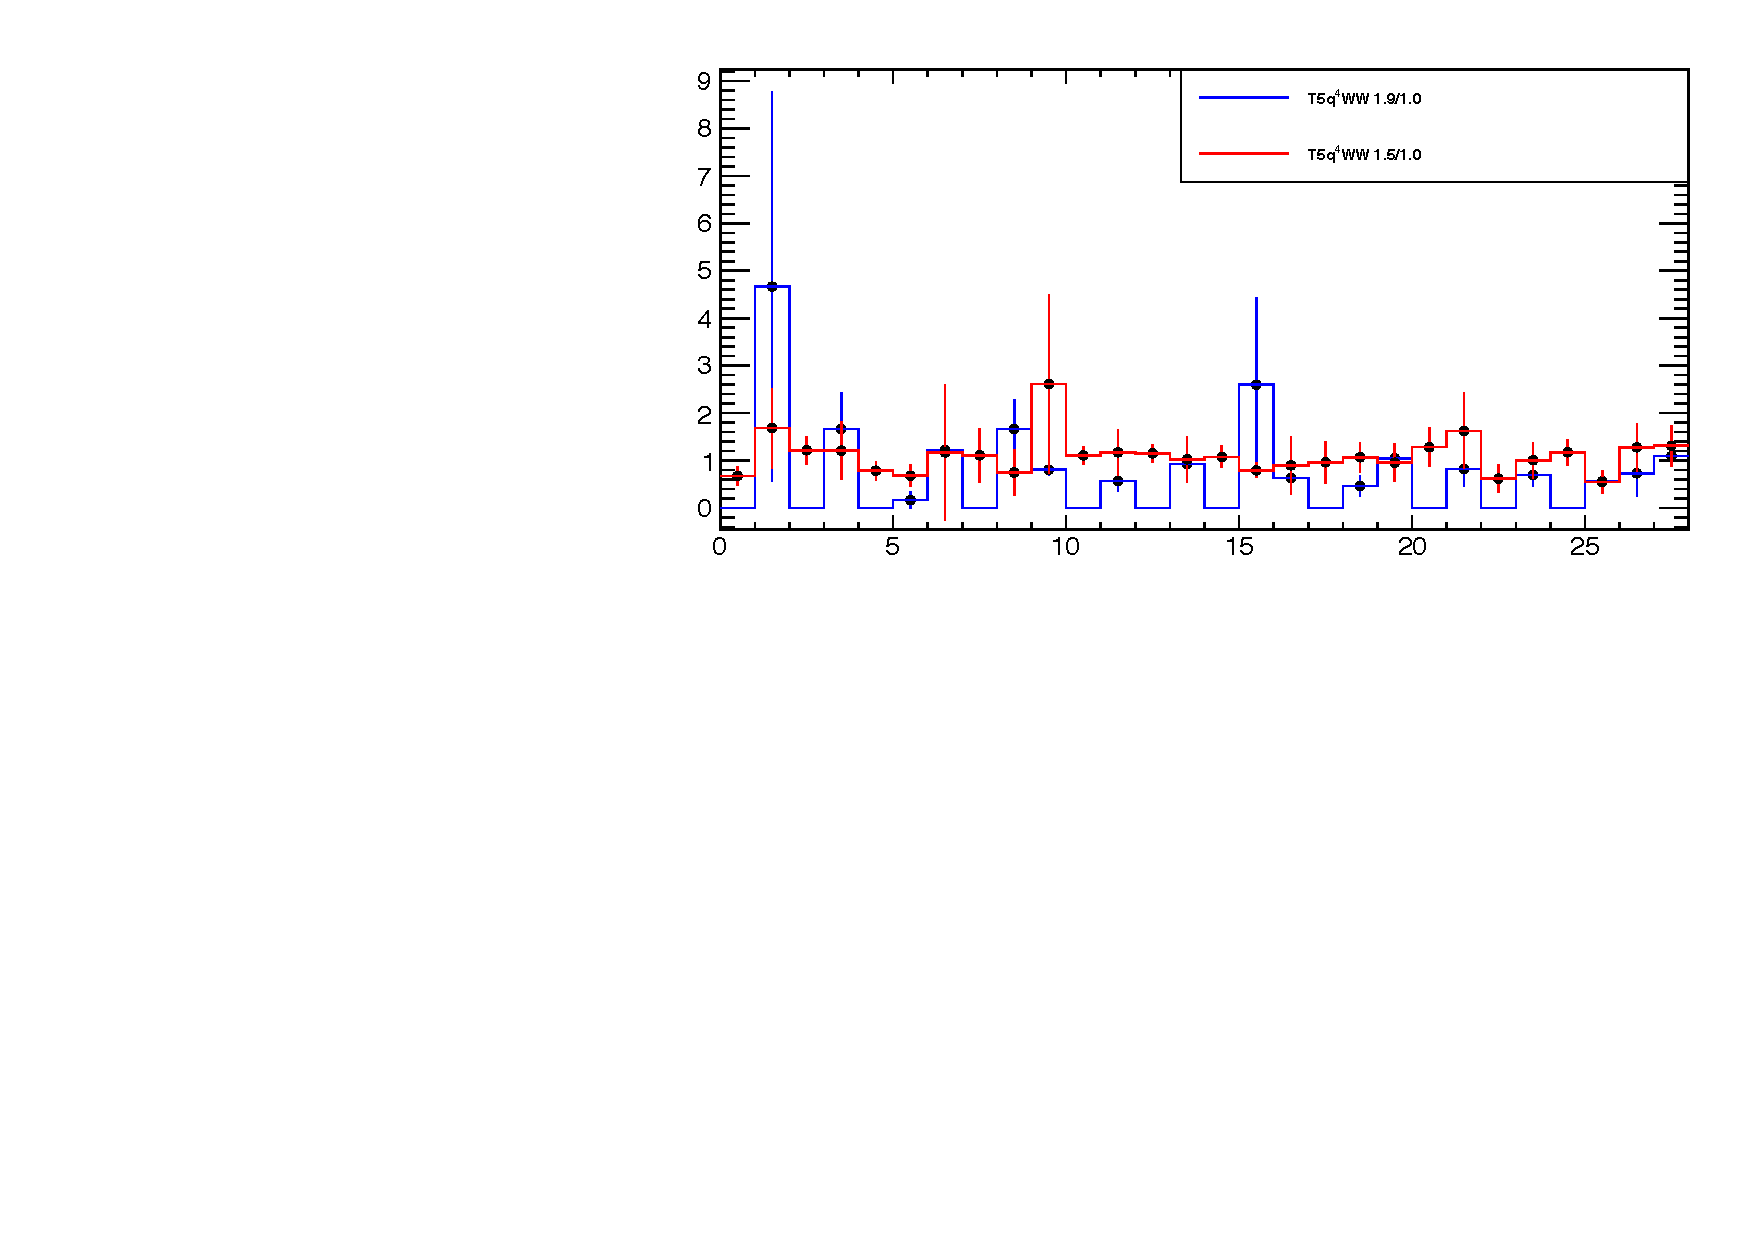
\includegraphics[width=0.8 \textwidth]{Plots/analysis/pileUp/PU_dependence}
  \caption{ \label{fig:pileUpdependence} Pileup dependence of the two signal benchmark points. The blue line is representing the hig mass gap point the red one is for low mass gap region. The histogram points are following a flat line around 1.}
  \end{center}
\end{figure*}
However, still an uncertainty has to be assigned to cover possible dependence. 
To drive an uncertainty, which is covering the differences between the simulated signal pileup distribution in main band regions and data, following steps have been followed. First, the signal sample is divided into a low and a high PU part according to mean value and then the mean values for each part is calculated as in Fig. \ref{fig:pileUpsystmech} (middle).
Second, the simulated efficiency in main band signal region is calculated for low and high pileup region as in Eqn. \ref{eff_PU}. Third, these four points, from first and second steps, together compose the two points in Fig. \ref{fig:pileUpsystmech} (right). A linear fit is performed to extrapolate for all the pileup range. Finally, normalized data pileup distribution is folded with the fit and the sum is calculated. 
This procedure is repeated by varying the two values from second step within their statistical uncertainties independently.
The relative difference to the central value is taken as uncertainty.
Then, the uncertainty is separately obtained for low and high pileup region and combined in to one by taking the squared sum of the two. The entire procedure is repeated for each mass point in the gluino-neutralino mass plane and for each main band region. The resultant uncertainty is found to be around 5-40\% depending on the statistics of the region for the corresponding mass point. In order not to double count the statistical errors, a 10\% flat uncertainty is applied to all bins for all mass points.\\
\begin{figure*}[!hbt]
    \begin{center}
  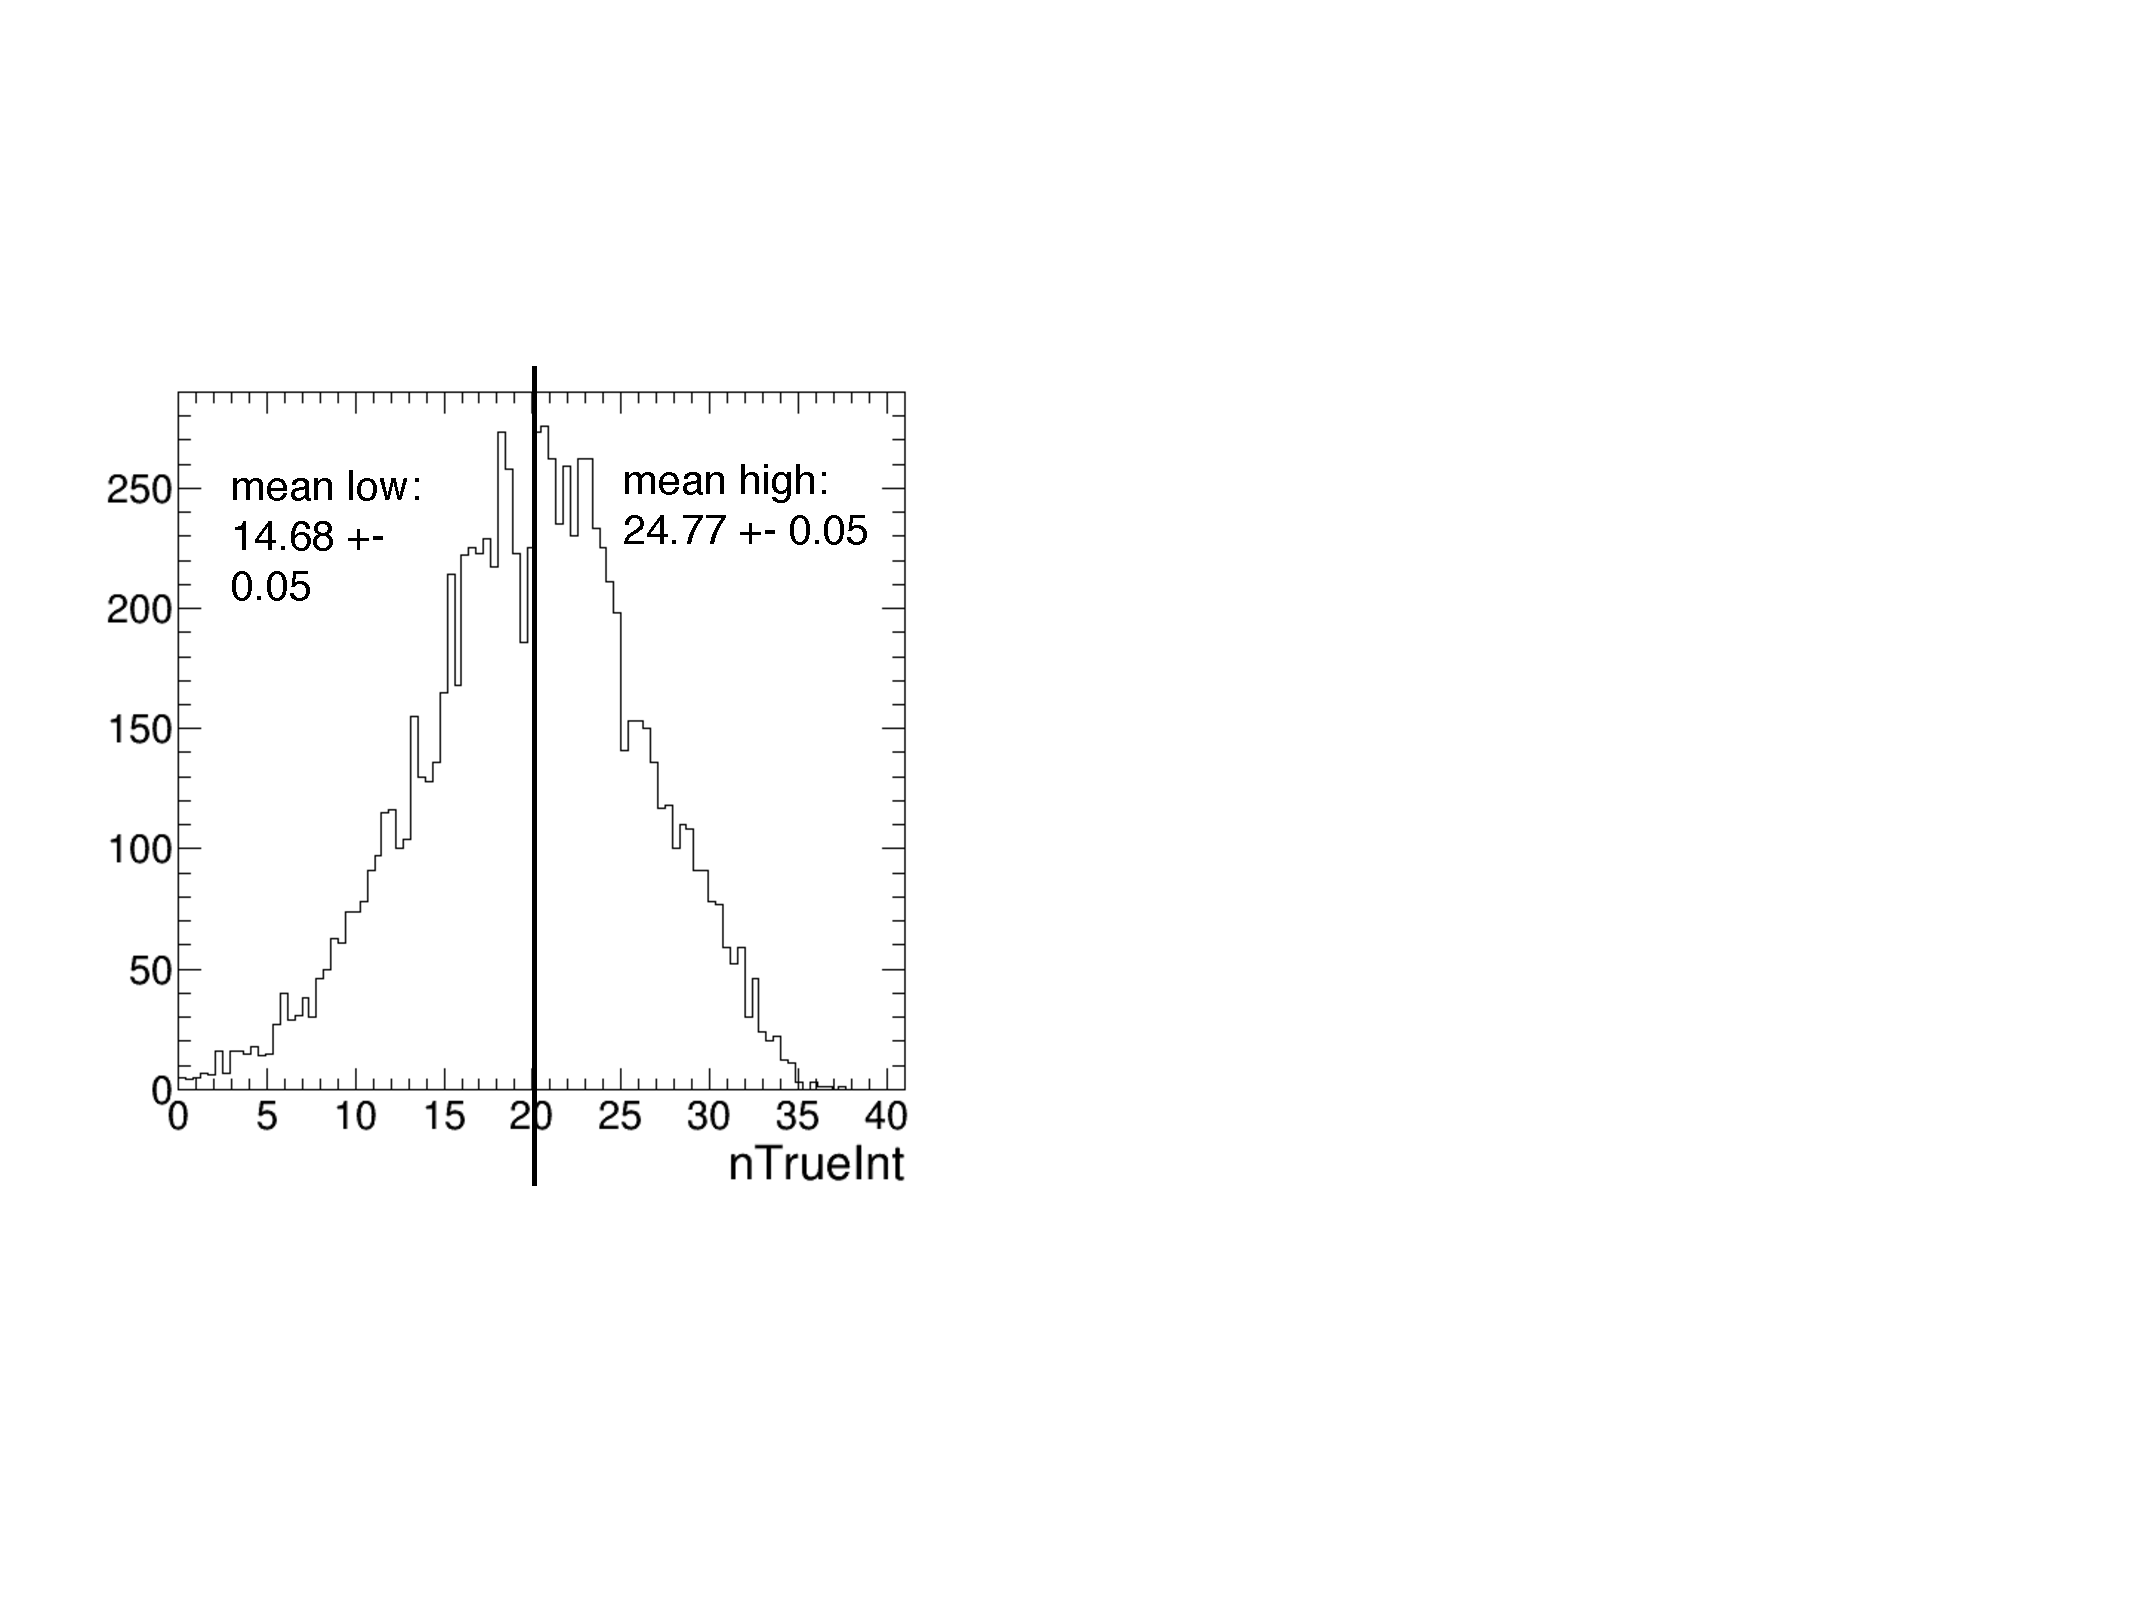
\includegraphics[width=0.3 \textwidth]{Plots/analysis/pileUp/lowmassgap_mean_forsyst}
   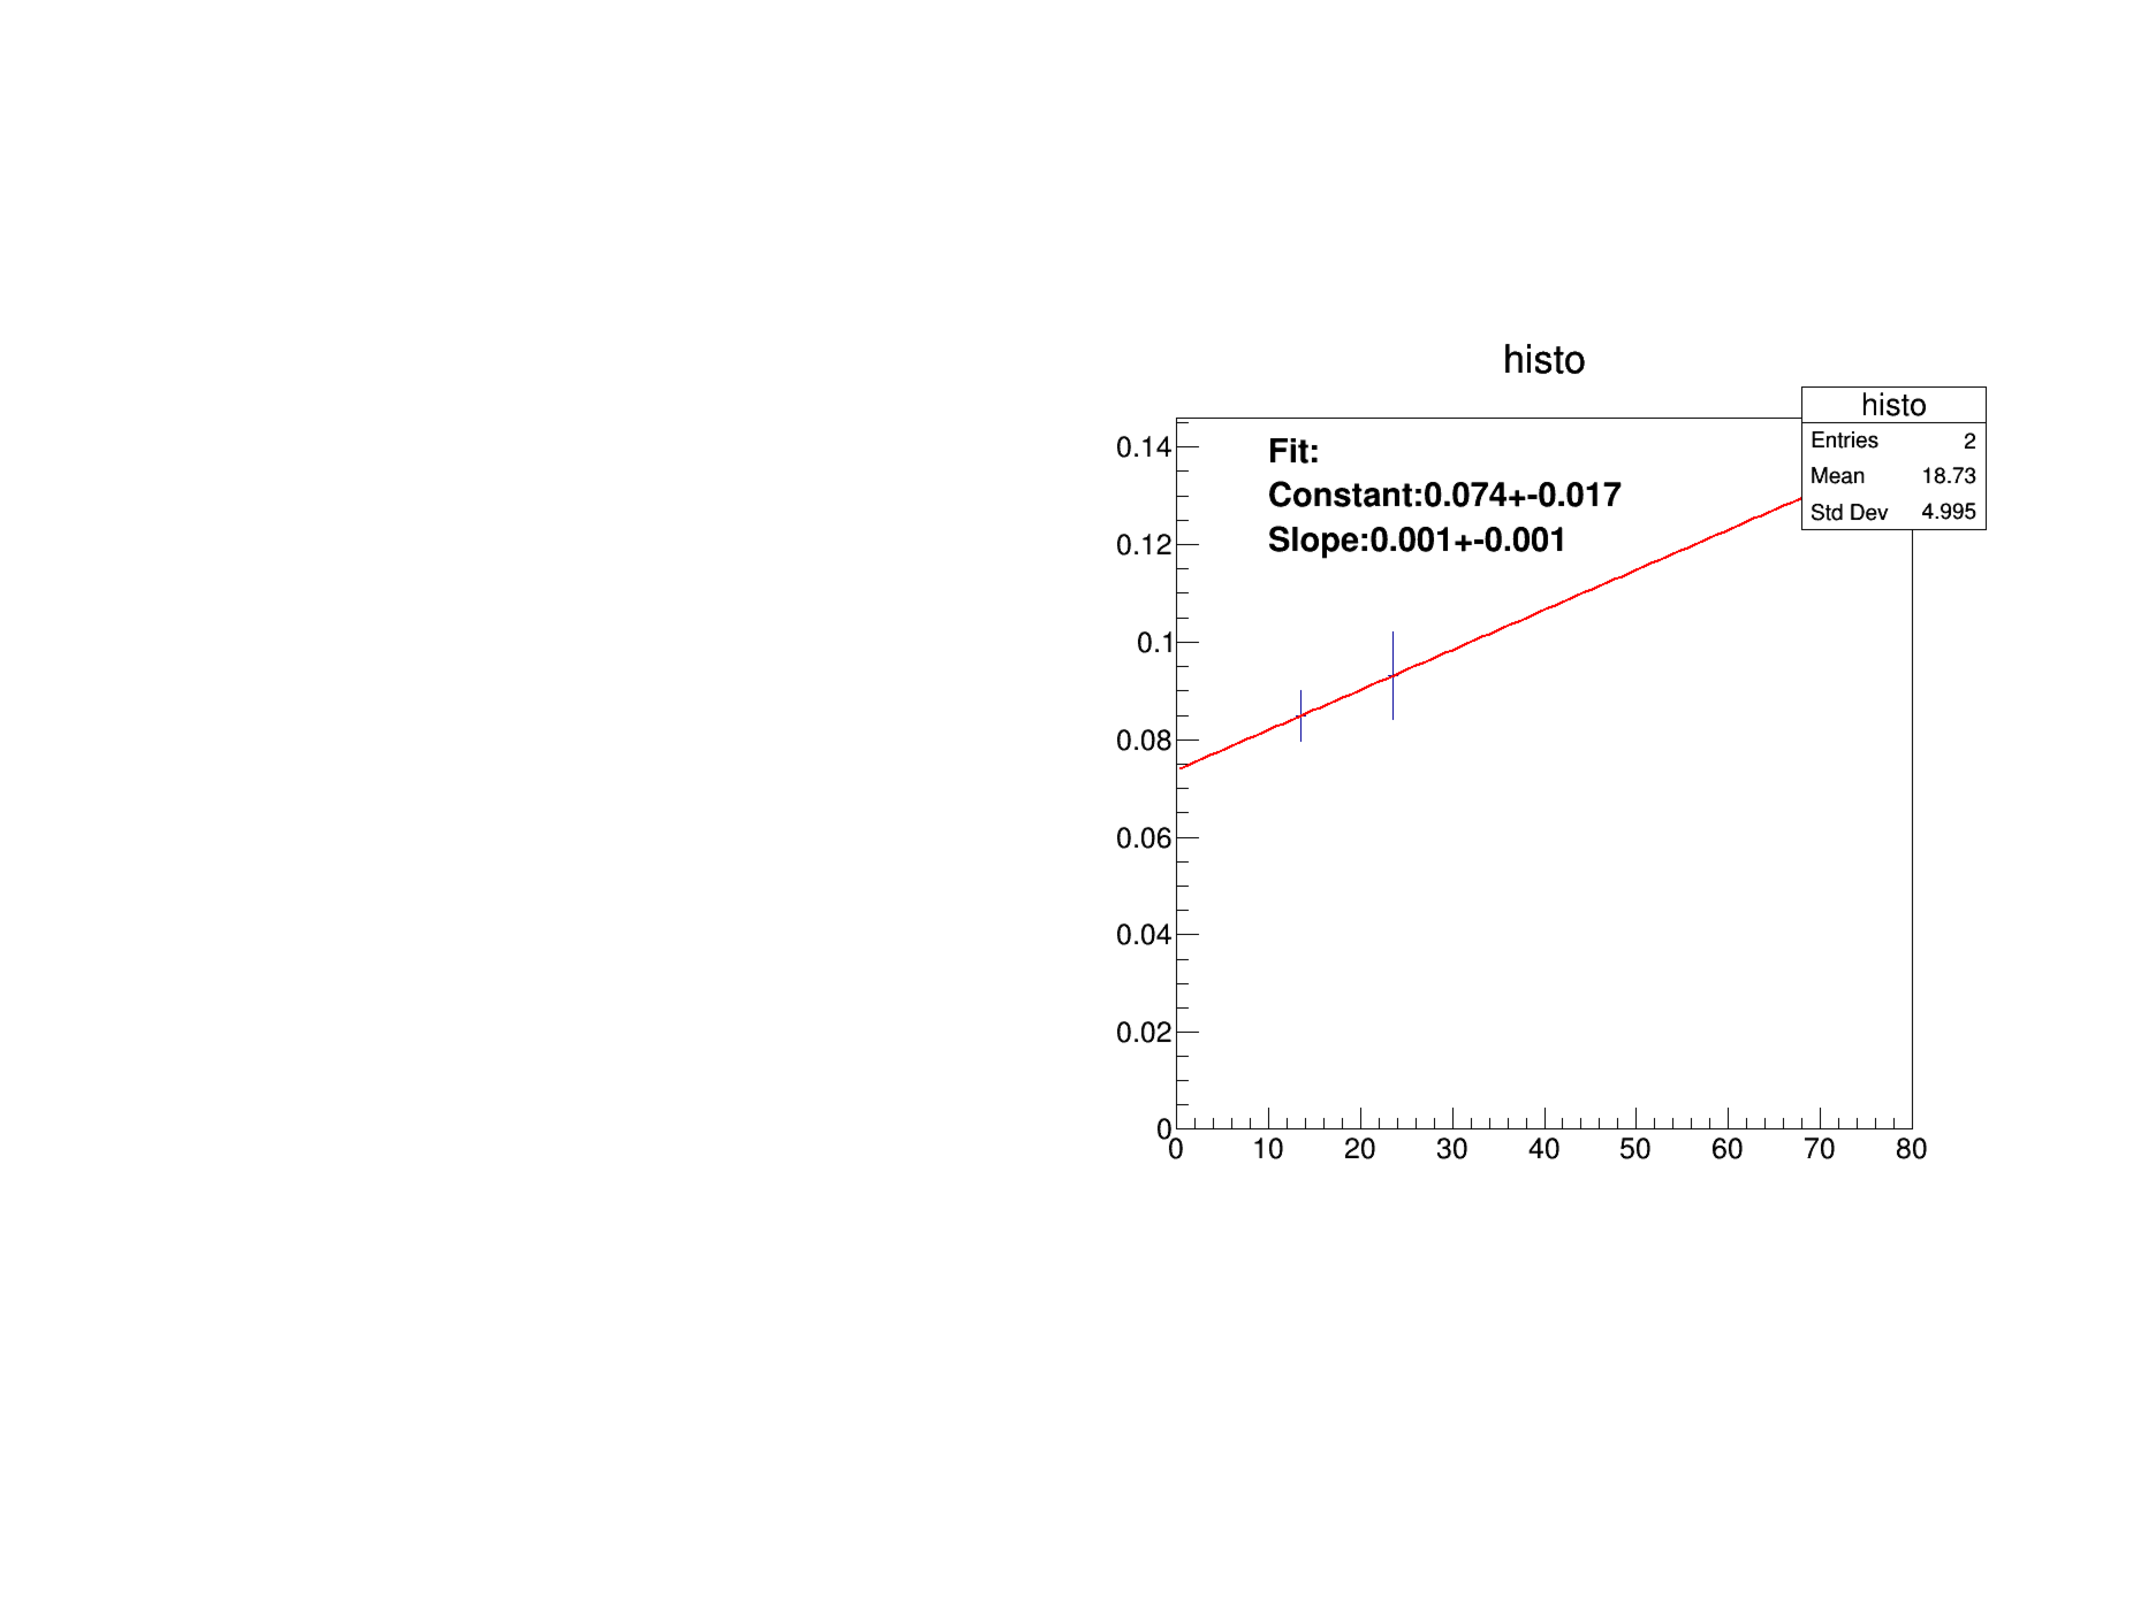
\includegraphics[width=0.3 \textwidth]{Plots/analysis/pileUp/fit_forsyst}
    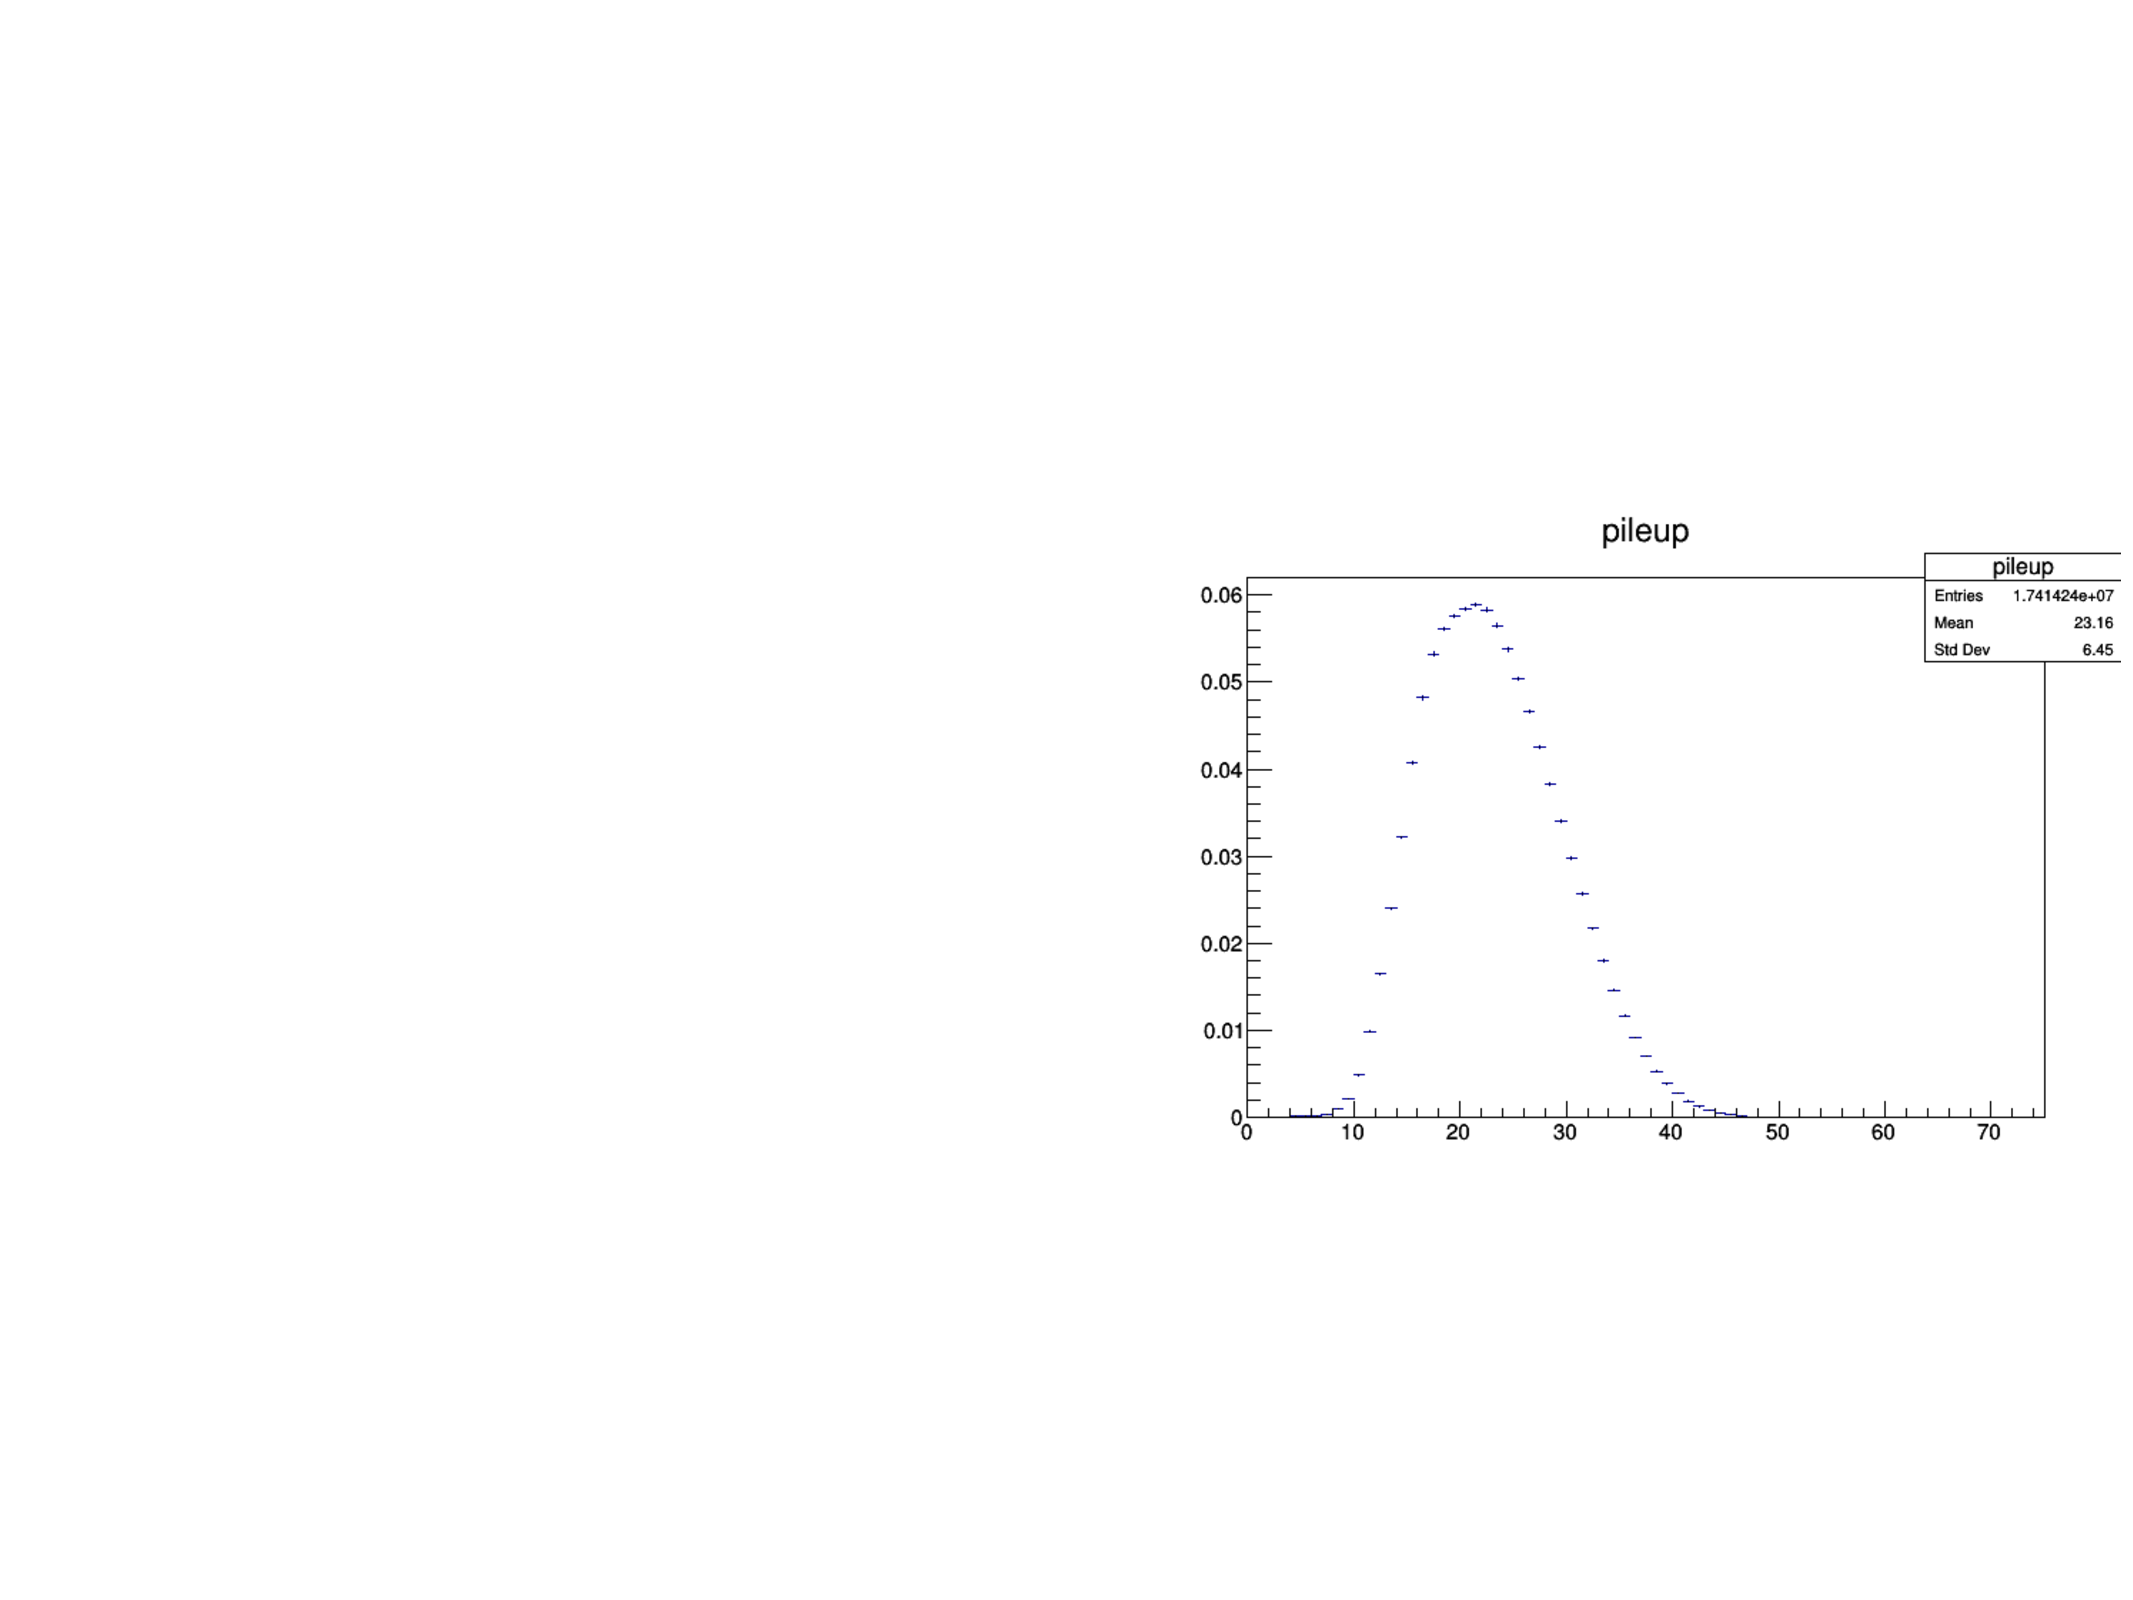
\includegraphics[width=0.3 \textwidth]{Plots/analysis/pileUp/datanorm_forsyst}
  \caption{ \label{fig:pileUpsystmech} Distribution of pileup for the high-mass gap signal sample, divided in to two parts as low and high pileup region (left), example fit performed using the two points examplained in the text (middle), data pileup  distribution which is folded with the fit.}
  \end{center}
\end{figure*}
\\
Fig. \ref{fig:systBKG} displays the different systematic uncertainties on the background prediction for main band signal regions while Fig. \ref{fig:systSig1} shows the systematic uncertainties on the simulated signal events for the mass point $m_{\tilde{g}}=$1900 and $m_{\ninoone}=$100. The total systematic uncertainty is calculated as the squared sum of all the different sources are shown with the black crosses and they are just for illustration. The total systematic uncertainty as well as statistical uncertainties is shown in the lower band of the two figures.\\
\begin{figure*}[!hbt]
    \begin{center}
  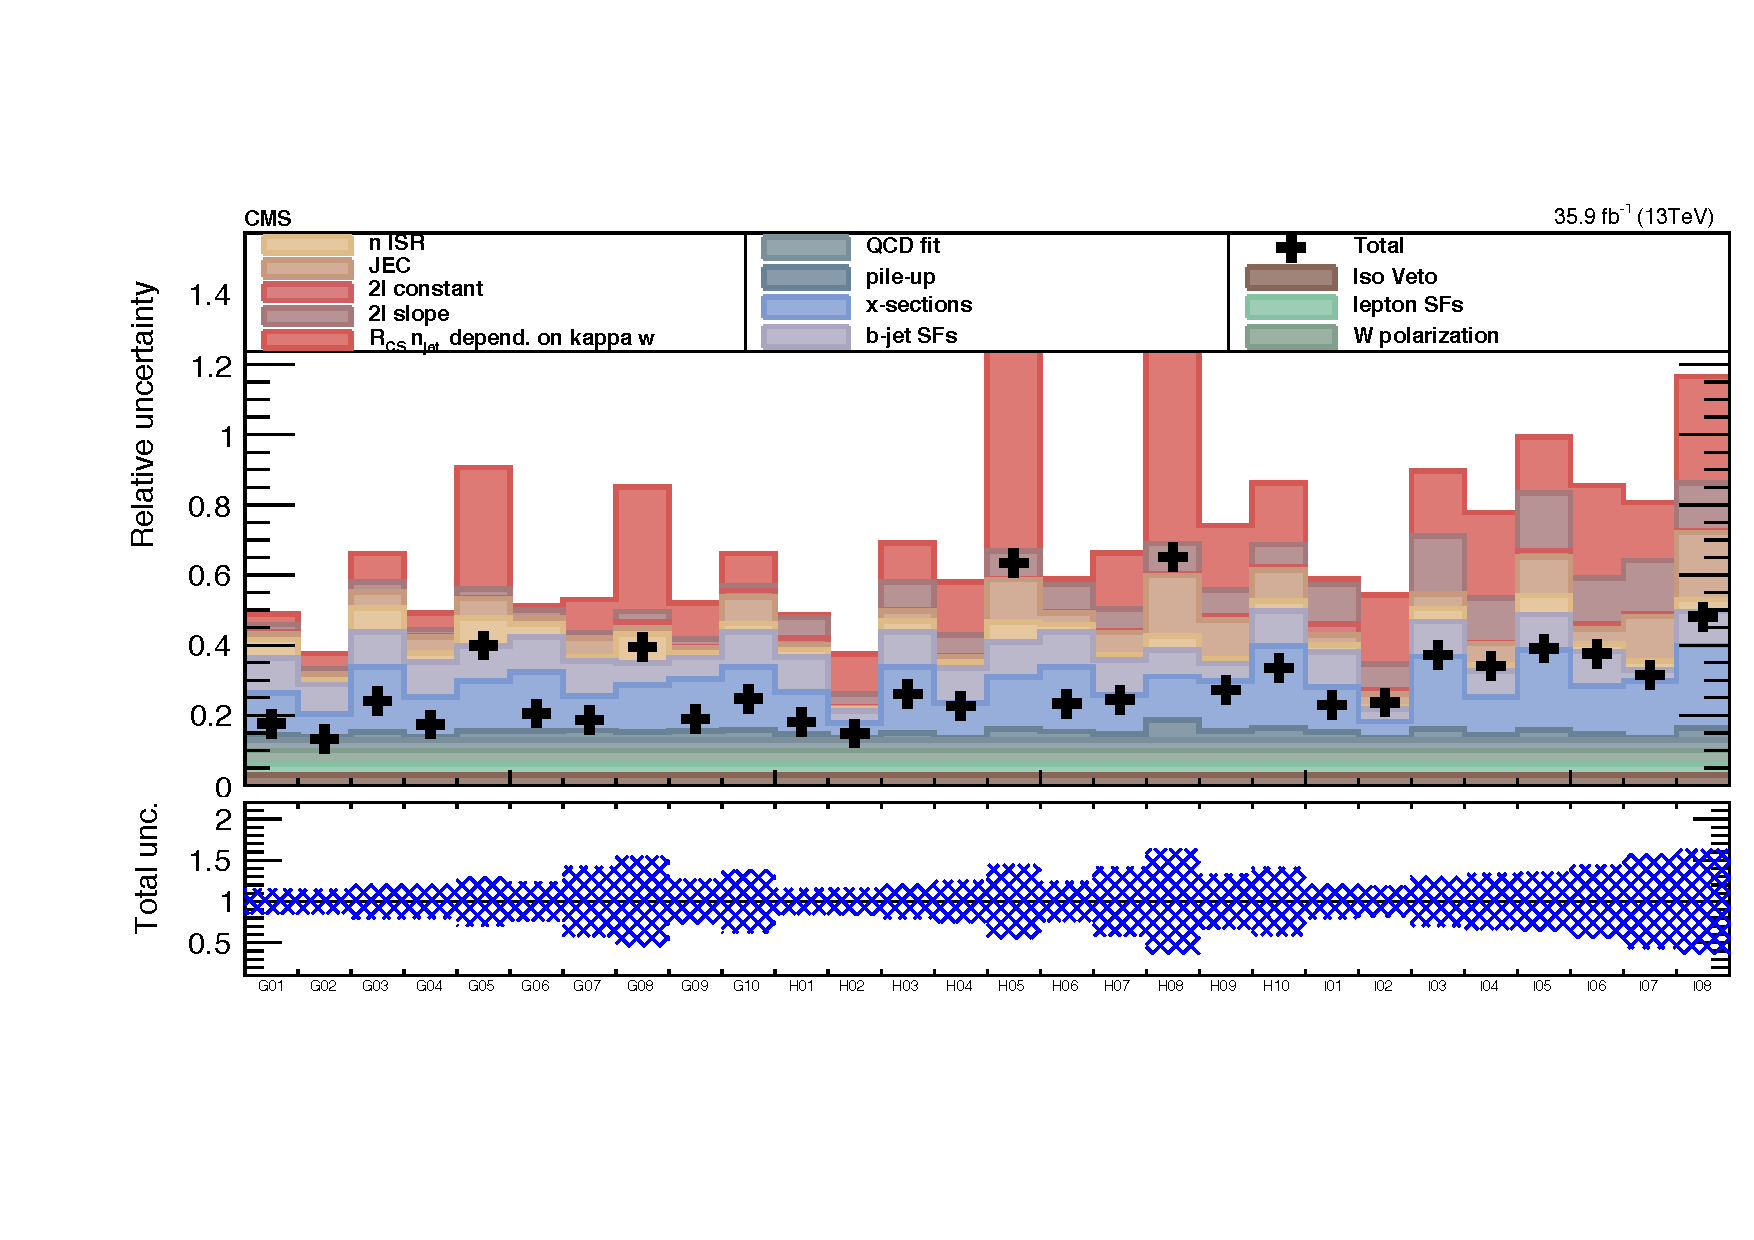
\includegraphics[width=0.8 \textwidth]{Plots/analysis/syst/plots_zerob_kappa_systematics_zerob}
  \caption{ \label{fig:systBKG} Visualization of all systematic uncertainties on the background prediction for main band regions described in Tab. \ref{tab:signal_regions}.}
  \end{center}
\end{figure*}
\begin{figure*}[!hbt]
    \begin{center}
  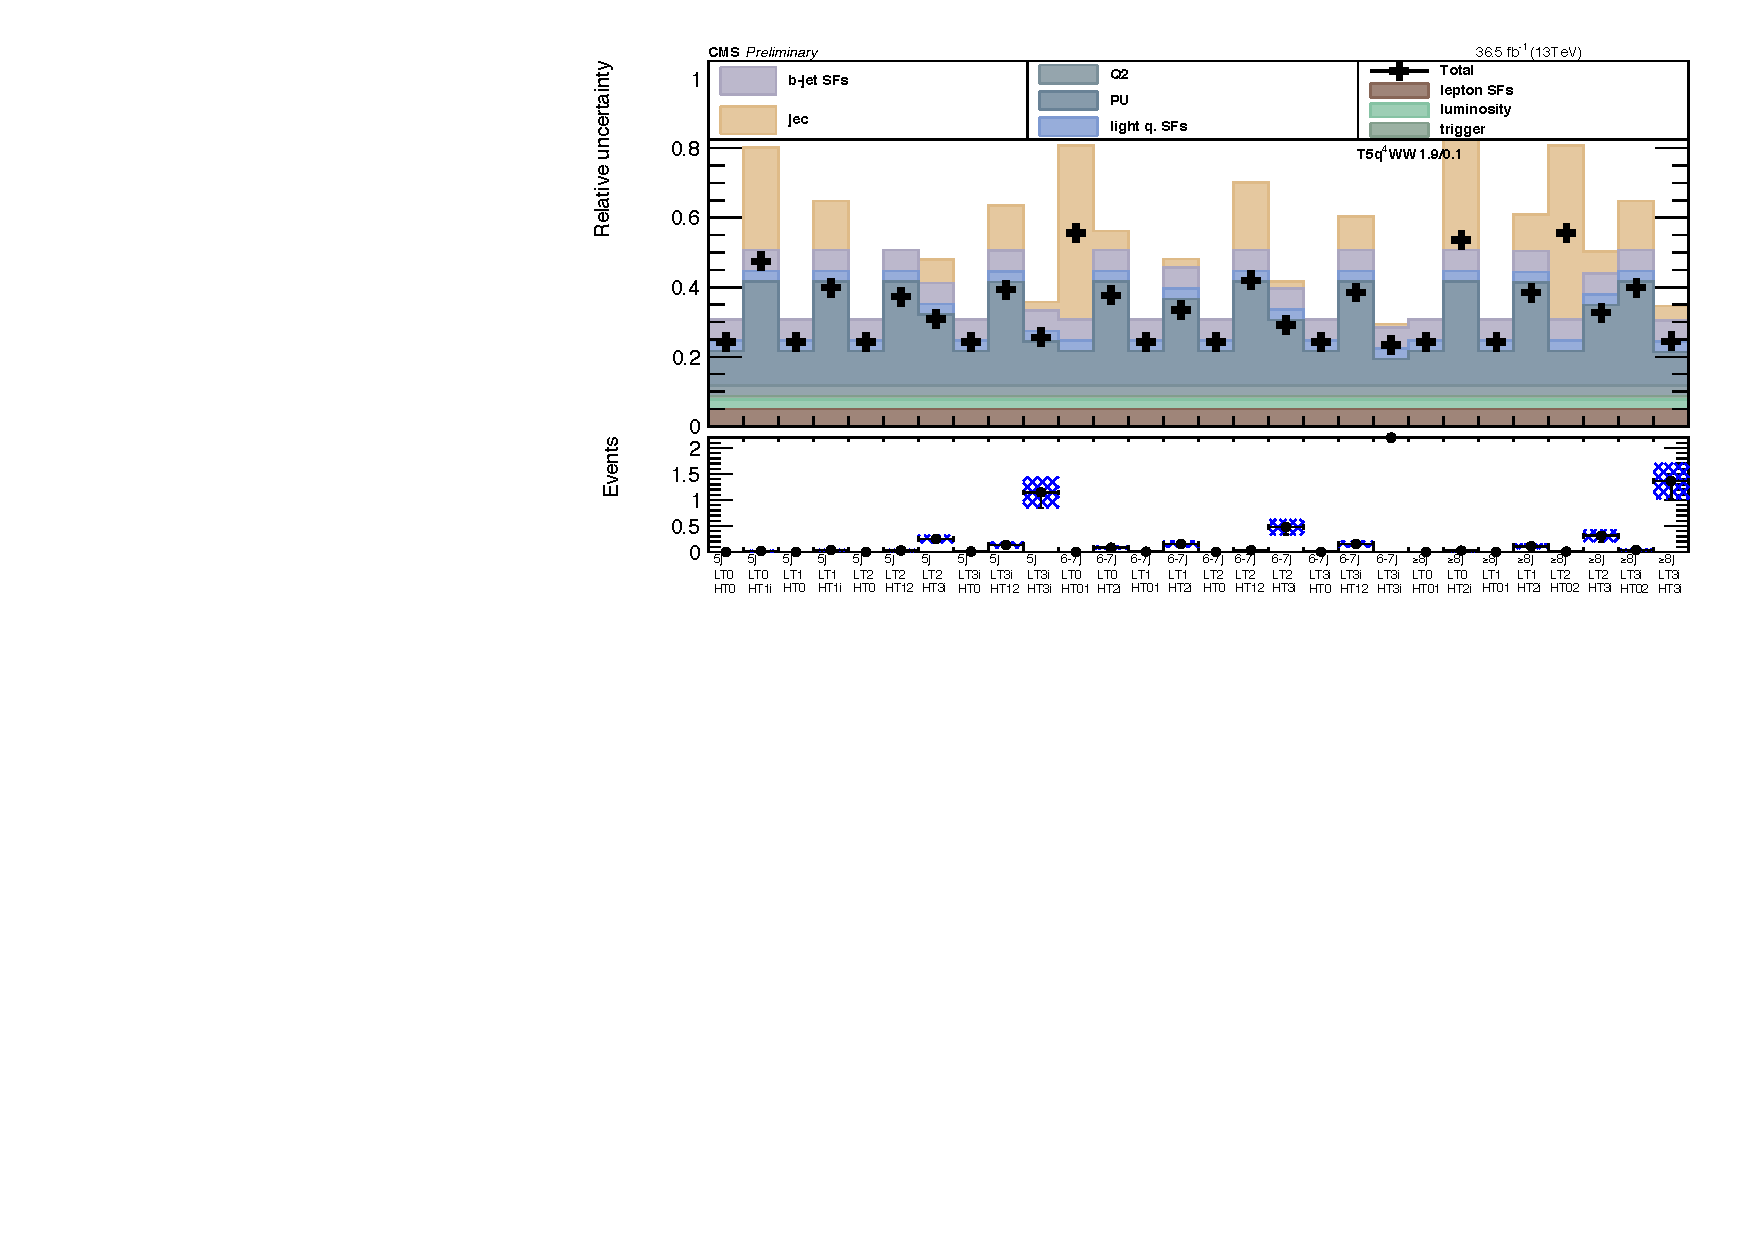
\includegraphics[width=0.9 \textwidth]{Plots/analysis/syst/syst_errors_signal_1900_100}
  \caption{ \label{fig:systSig1} Visualization of all systematic uncertainties on the simulated signal yields in main band regions described in Tab. \ref{tab:signal_regions}. Uncertainities are shown only for one mass point which is  $m_{\tilde{g}}=$1900 and $m_{\ninoone}=$100. }
  \end{center}
\end{figure*}
